\chapter{Limit state design methods of Hybrid Connection}
\label{ch7}

%%%%%%%%%%%%%%%%%%%%%%%%%%%%%%%%%%%%%%%
% IMPORTANT
\begin{spacing}{1.25} %THESE FOUR
\minitoc % LINES MUST APPEAR IN
\end{spacing} % EVERY
\onehalfspacing % CHAPTER
% COPY THEM IN ANY NEW CHAPTER
%%%%%%%%%%%%%%%%%%%%%%%%%%%%%%%%%%%%%%%


% 列出两种模型 一个是有小滑移的,一个是没有小滑移的理想状态,然后基于理想状态进行耐力折减,耐力可以定义在非线性前,

\section{Introduction}

In recent years, high-strength bolts have partially replaced aging rivets, resulting in a combination of the bearing type connection and a friction connection between rivets and high-strength bolts on the same joint. On the other hand, in the construction of new bridges, tendency for component to be designed in larger sizes and use of high-strength steel has led to the challenge of providing high resistance joints with limited bolts. To address this challenge, a hybrid joint design has been proposed which combines bearing type and friction type connections. This approach can improve joint strength without significantly increasing construction complexity. However, the differentiation of the limit states of hybrid connections has not been discussed in detail. This chapter will use numerical analyses and experimental verification to discuss limit states of hybrid joints and propose a strength calculation formula based on bearing resistance.

% 由于摩擦连接的刚度和承压连接不同,当共同作用在一个连接中时,在弹性范围内会出现一次斜率的改变,这是由于接头由摩擦传递为主转变为以承压传递为主导致的,但是研究认为这不会影响连接的承载力。日本的JSHB规定了承压连接的使用极限状态,是基于强度设计的,且考虑了承压连接的刚度,允许接头有一定的变形能力,因此,对于混合接头的极限状态设计,可以同时考虑承压连接和摩擦连接的极限状态设计方法,也就是在确保了承压连接的强度的前提下,考虑摩擦连接的刚度控制接头的变形量,从而得到混合连接的极限状态设计方法。
% 对于混合连接的极限状态设计,主要考虑的是连接的承载力,即连接的耐力。在第\ref{ch6}章中,我们已经得到了混合连接的耐力计算公式,但是这个公式是基于理想状态的,即连接中没有小滑移。在实际的连接中,由于连接的刚度有限,连接中会产生一定的小滑移,这个小滑移会影响连接的承载力。因此,本章将基于第\ref{ch6}章的理论,对混合连接的极限状态设计方法进行探讨。
% 由于混合连接的承载力设计是基于理想状态的,因此,本章将首先对理想状态下的混合连接进行极限状态设计,然后再考虑小滑移对连接承载力的影响,提出一个基于小滑移折减系数,最后得到混合连接的极限状态设计方法。

Since the stiffness of friction connections is different from that of bearing connections, when acting together in a connection, there will be a change in slope once in the elastic range, which is caused by the change of the joint from friction transfer to predominantly bearing transfer, but the study concludes that this will not affect the load carrying capacity of the connection. Japan's JSHB stipulates the limit state of bearing connections, which is based on bearing resistance, and takes into account the stiffness of the bearing connection, allowing the joint to have a certain amount of deformation, therefore, for the limit state design of hybrid joints, the limit state design method of both bearing resistance and friction joints can be considered at the same time, that is, under the premise of ensuring the strength of the bearing resistance connection, the stiffness of friction joints is taken into account to control the deformation of the joints. In other words, under the premise of ensuring the strength of the compression connection, the stiffness of the friction connection is taken into account to control the deformation of the joint, thus obtaining the limit state design method of hybrid connection.

For the limit state design of hybrid connection, the main consideration is the bearing capacity of the connection, i.e. the endurance of the connection. In Chapter \ref{ch6}, we have obtained the formula for calculating the endurance of the hybrid connection, but this formula is based on the ideal state, i.e., there is no small slip in the connection. In the actual connection, due to the limited stiffness of the connection, there will be a certain small slip in the connection, and this small slip will affect the load carrying capacity of the connection. Therefore, this chapter will discuss the limit state design method of hybrid connection based on the theory in Chapter \ref{ch6}.

Since the design of the load carrying capacity of the hybrid connection is based on the ideal state, this chapter will firstly carry out the limit state design of the hybrid connection in the ideal state, and then consider the influence of small slip on the load carrying capacity of the connection, propose a small slip discount factor based on it, and finally obtain the limit state design method of the hybrid connection.

\section{Mechanic behavior of Hybrid Connection}

\subsection{Friction type connection}

Since the hybrid connection is composed of a bearing connection and a friction connection, the stiffness of the hybrid connection is determined jointly by the stiffness of the bearing connection and the friction connection. Before calculating the limit state design method for the hybrid connection, the stiffness of the friction connection needs to be calculated first.

\begin{figure}[htbp]
    \centering
    \includegraphics[width=0.8\textwidth]{imgs/ch7/RBSM.pdf}
    \caption{Rigid body-spring model of friction type connection}
    \label{fig-rbsm}
\end{figure}

The stiffness model of the friction connection can be simplified to the model shown in Fig. \ref{fig-rbsm}, where $k_{s}$ is the stiffness of the friction connection, $k_{e}$ is the stiffness of the steel plate considering the circular holes, and the equations for $k_{s}$ and $k_{e}$ are as follows:

\begin{equation}\label{eq-ks}
    K_{s} = 8GA_{se} \varphi / (t + 2 t_{sp})
\end{equation}

Where, $G$ is the shear modulus, $A_{sq}$ is the effective area of the friction connection, $t$ is the thickness of the main plate, $t_{sp}$ is the thickness of the splice plate, and $\varphi$ is the correction coefficient of shear strain, The geometry of the cut micro-unit and the range of friction influences are determined by taking 0.5 for the case of M22 bolts and 28 mm splice plate thickness for this object.

\begin{figure}[htbp]
    \centering
    \includegraphics[width=0.8\textwidth]{imgs/ch7/simp_rbsm.pdf}
    \caption{Simple RBSM model under simple shear}
    \label{fig-simp_rbsm}
\end{figure}

As the high-strength bolts through the washer to transfer the clamping force to the friction joint surface as shown in Fig. \ref{fig-simp_rbsm}, so in the consideration of the shear area should be brought into the area of the washer to be considered together, in addition, the actual contact surface pressure range is larger than the washer area, so it is necessary to consider the influence due to the shear strain effect by multiplying a correction coefficient $\psi$ on the washer area $d_w$.
Therefore As can be calculated with the following equation:

\begin{equation}
    A_{se} = \pi{(\psi d_w)^2-d_0^2} / 4
\end{equation}

Where, $d_0$ is the diameter of the bolt hole, and $\psi$ is the correction coefficient of contact area, in the case of thin plates take 1, in the case of thick plates it can be simply taken as 1.4.

\subsubsection{Validation of stiffness calculation}

In order to verify the correctness of the stiffness calculation of the friction connection, the stiffness of the friction connection is calculated by the above formula, and the stiffness of the friction connection is calculated by the Eq. \ref{eq-ks}, and the results are compared with the Chapter 6. 

For the hybrid joint, M22 bolts were used at the end and M16 bolts were used in the middle, and the stiffness of the joint was mainly controlled by the M22 bolts at the end, so when the calculation was carried out, it was agreed to follow the geometry of the M22 bolts at the end in order to facilitate the simplification of the model, and the details of the calculation are shown in Table \ref{tab-calks}.

\begin{table}[]
    \centering
    \caption{Calculation of stiffness of friction type connection}
    \label{tab-calks}
    \begin{tabular}{@{}cccccccc@{}}
    \toprule
     &
      \begin{tabular}[c]{@{}c@{}}Shear Modulus\\ G {[}Gpa{]}\end{tabular} &
      $\psi$ &
      \begin{tabular}[c]{@{}c@{}}$d_w$\\ {[}mm{]}\end{tabular} &
      \begin{tabular}[c]{@{}c@{}}$d_0$\\ {[}mm{]}\end{tabular} &
      \begin{tabular}[c]{@{}c@{}}$A_{se}$\\ {[}$mm^2${]}\end{tabular} &
      $\varphi$ &
      \begin{tabular}[c]{@{}c@{}}$K_s$\\ {[}$kN/mm${]}\end{tabular} \\ \midrule
    M22-bolt &
      77 &
      1.4 &
      44 &
      23.5 &
      2550 &
      0.5 &
      10069.5 \\ \bottomrule
    \end{tabular}
\end{table}

The initial frictional stiffness ks of this hybrid joint is calculated to be 10069 kN/mm. It is assumed here that the friction tends to be horizontal and does not change after sliding of the joint, which is in agreement with the finite element simulation, and therefore the slope is changed to 0 after sliding load. The friction connection can be modeled as the following equation

\begin{equation}\label{eq-nmfc}
    P = \begin{cases}
        K_s \delta, & \text{if } P < F_{s} \\
        F_{s}, & \text{if } P \geq F_{s}
    \end{cases}
\end{equation}

Fig.\ref{fig-ks_compare} represents the comparison made with this model and the experimental results, where NA-FC denotes the numerically Analysis-friction type Connection indicated by the dashed line. This model can be considered as a good simulation of the variation of friction in the joint without considering the preload drop of the bolt.

\begin{figure}[htbp]
    \centering
    \includegraphics[width=0.7\textwidth]{imgs/ch7/NA-FC.eps}
    \caption{Comparison of stiffness of friction type connection}
    \label{fig-ks_compare}
\end{figure}

\subsection{Bearing type connection}

%对于承压连接,虽然规定了采用承压强度设计时可以不用施加轴力,然而一般设计为了提高刚度和强度,都会对用于承压连接的螺栓施加轴力。这使得承压连接自身就分为了两种状态,一种是不施加轴力的承压连接,一种是施加轴力的承压连接。对于不施加轴力的承压连接,其刚度可以直接通过螺栓的刚度计算得到,而对于施加轴力的承压连接,其刚度需要通过螺栓的剪切和摩擦刚度计算得到。对于,摩擦连接的刚度计算方法已经在上一节中进行了介绍. 因此为了更简单的讨论复合作用下的承压连接的刚度,本节将首先讨论不施加轴力的承压连接的刚度计算方法,然后再讨论施加轴力的承压连接的刚度计算方法。

For pressurized connections, although it is stipulated that no preload can be applied when designing for bearing resistance, the bolts used for pressurized connections are generally designed to apply preload in order to increase stiffness and strength. This makes the bearing connection itself divided into two states, one is the bearing connection without preload, and the other is the bearing connection with preload. For a bearing connection without preload, the stiffness can be calculated directly from the stiffness of the bolts, whereas for a bearing connection with preload, the stiffness needs to be calculated from the shear and friction stiffness of the bolts. For, the stiffness calculation method for friction connections has been described in the previous section. Therefore in order to discuss the stiffness of compression connections under composite action in a simpler way, this section will first discuss the method of calculating the stiffness of compression connections without applied pretension and then the method of calculating the stiffness of compression connections with applied pretension.

\begin{figure}[htbp]
    \centering
    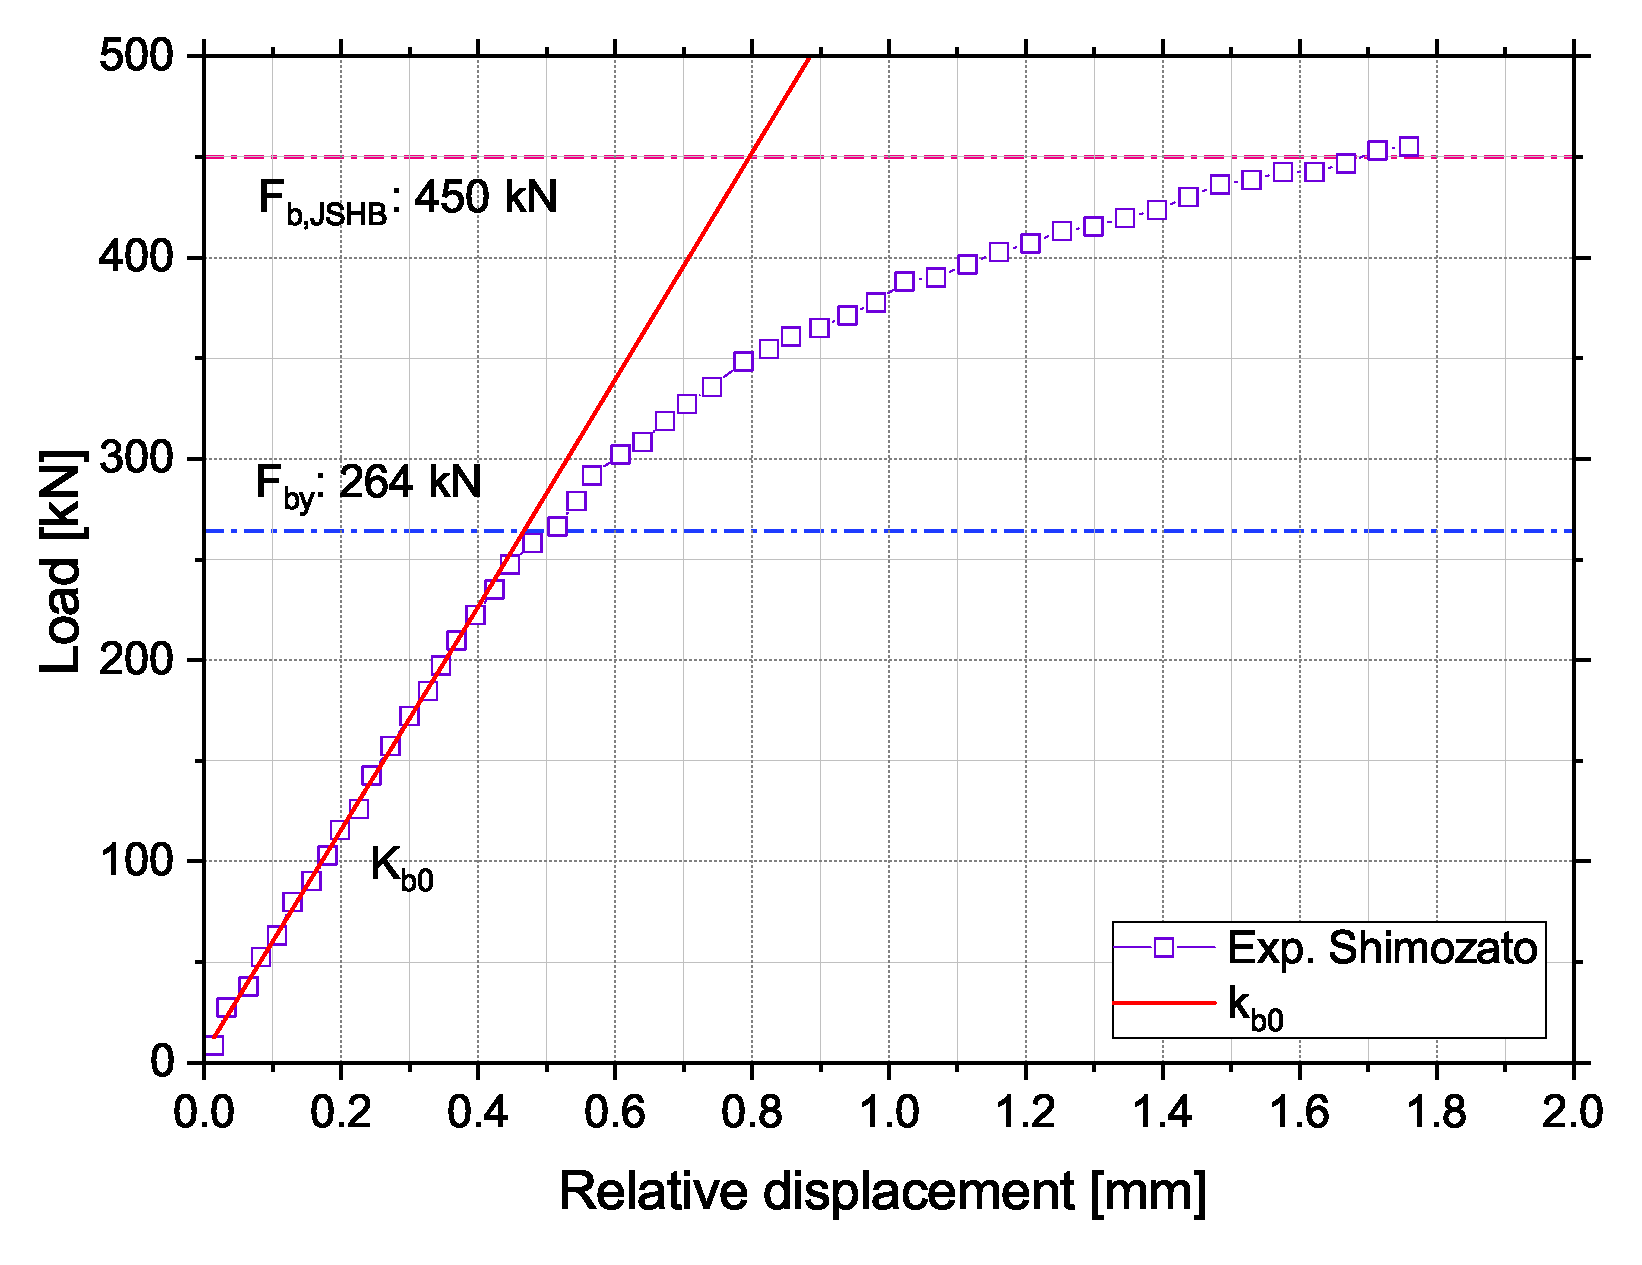
\includegraphics[width=0.7\textwidth]{imgs/ch7/onebbolt.eps}
    \caption{Bearing type connection without pretension}
    \label{fig-onebbolt}
\end{figure}

Fig. \ref{fig-onebbolt} shows the relationship between load and relative displacement for an if bolt subjected to shear with no preload applied. The data were obtained from shimozato's \cite{Shimozato2008ExperrimentalModel} experimental results, and it can be calculated from the experimental results that the bearing connection has an initial stiffness kb0, and the bearing resistance at the service limit strength obtained by the jshb calculation is 450 kN. It has also been mentioned in the previous Chapters \ref{ch4} and \ref{ch6}, respectively, that for the design at the service limit state, the stress-training effect should not be taken into account around the bearing holes, and thus the bearing bearing considered in this study bearing yield resistance $F_{by}$ should be calculated by the following equation:

\begin{equation} \label{eq-fby}
    F_{by} = dtf_y
\end{equation}

The bearing yield resistance obtained from Eq. \ref{eq-fby} is 264 kN, which can be found to be similar to the point in the experimental data where the linear relationship is removed. (purple dotted line and red solid line in the figure)

\subsection{Hybrid connection}

\subsubsection{Simplified theoretical numerical model}

\begin{figure}[htbp]
    \centering
    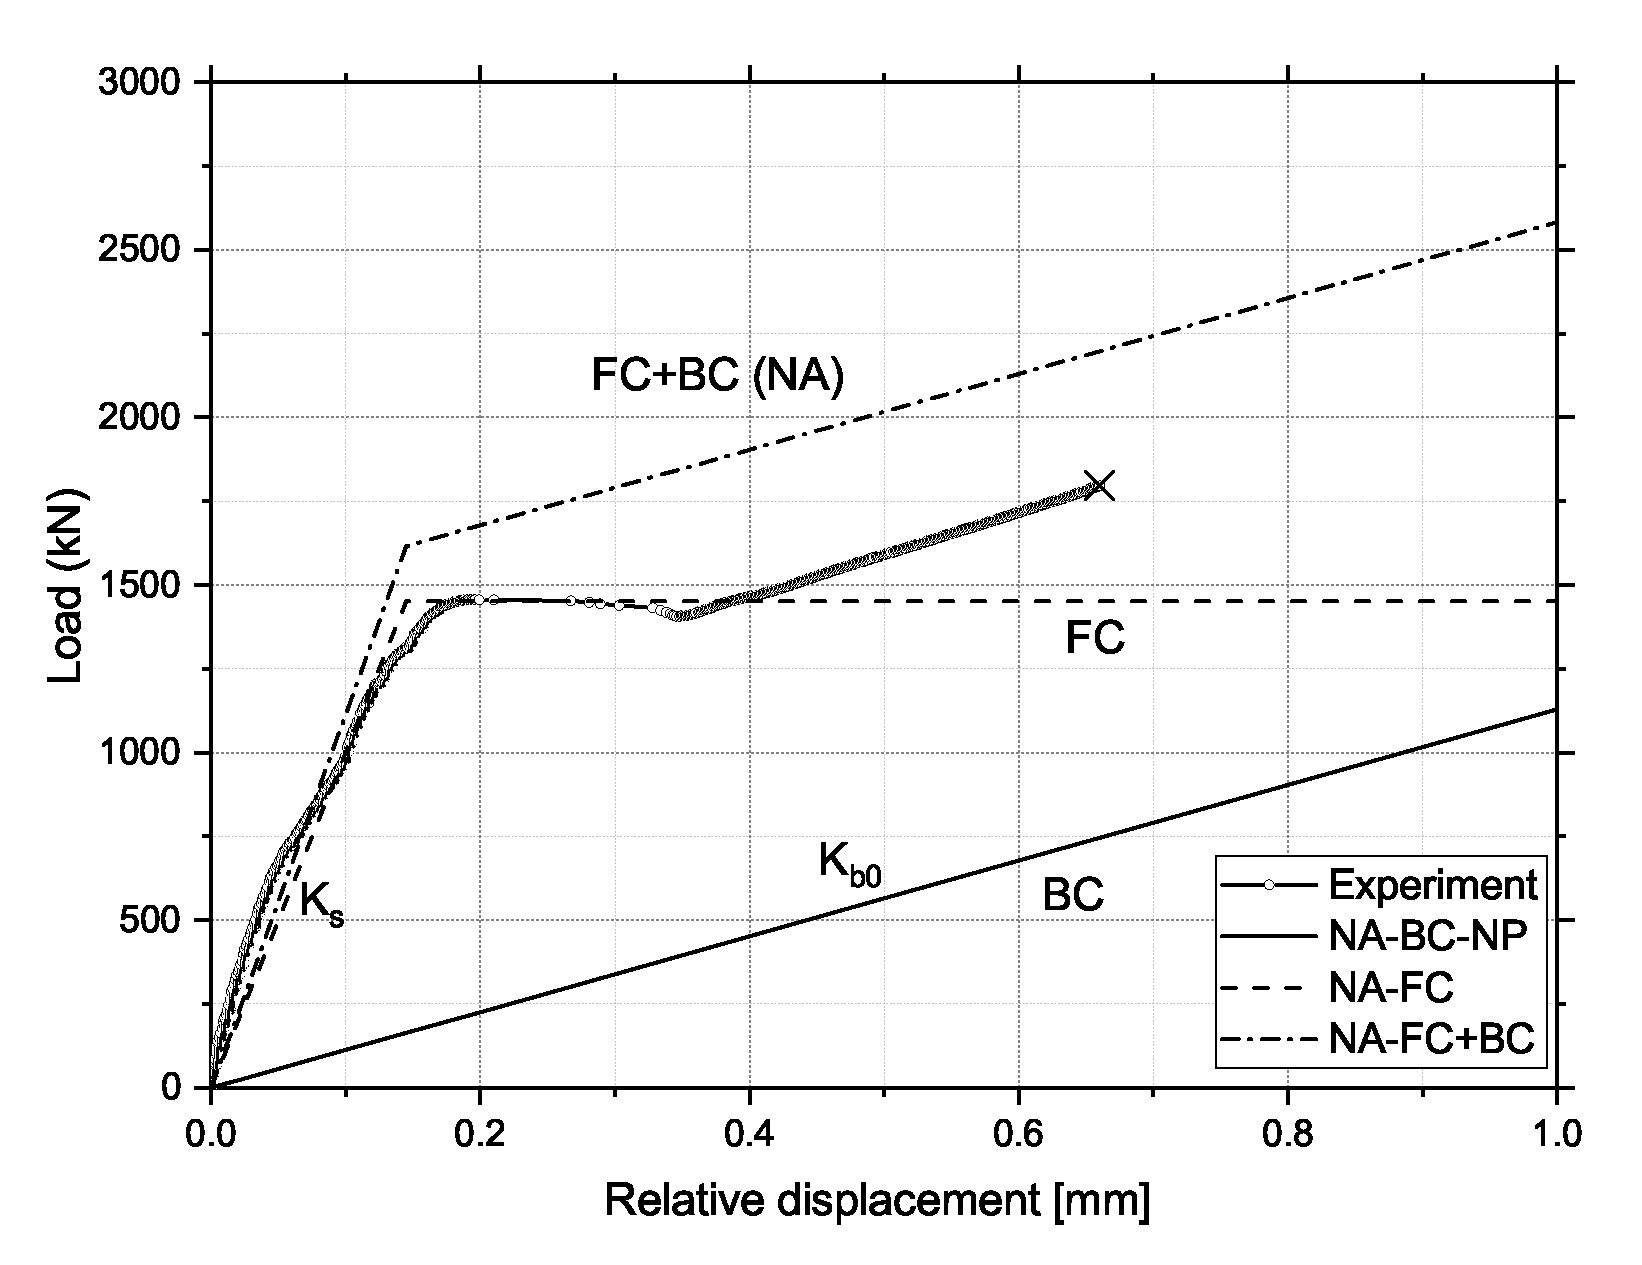
\includegraphics[width=0.7\textwidth]{imgs/ch7/NAFCBC.eps}
    \caption{Simplified theoretical numerical model of hybrid connection}
    \label{fig-nafcbc}
\end{figure}

Fig. \ref{fig-nafcbc} shows the simplified theoretical numerical model obtained by direct summation of the bearing and friction connections, the solid line of BC indicates the initial stiffness of the bearing connection, and the FC is modeled as shown in Eq. \ref{eq-nmfc}. The numerical model obtained by summation can be calculated by the following equation:

\begin{equation}\label{eq-nmhc1}
    P = \begin{cases}
        (K_s + K_{b0}) \delta, & \text{if } P < F_{s} \\
        K_{b0} \delta + F_{s}, & \text{if } P \geq F_{s}
    \end{cases}
\end{equation}

The numerical model simulates only the linear behavior of the hybrid connection, and it can be found that the model has a tendency to have roughly the same behavior as the experimental data for both the primary and secondary slopes, respectively, which can be considered appropriate assuming that no small slips will ideally occur.

\subsubsection{Consider the minor slip}

\begin{figure}[htbp]
    \centering
    \includegraphics[width=0.7\textwidth]{imgs/ch7/nmfcbc-2.eps}
    \caption{Corrected theoretical numerical model of hybrid connection with minor slip}
    \label{fig-nmfcbc2}
\end{figure}

Fig. \ref{fig-nmfcbc2} represents the model after correction for minor slips based on the base model Eq. \ref{eq-nmhc1}. Considering that at the initial stage of loading, although the bearing will transmit the load together with the friction connection, its load sharing is very small, especially since the initial stiffness of the hybrid connection is almost exclusively affected by the stiffness of the friction connection, this model does not take into account the bearing connection at the initial stage of the friction connection, which is summed up after the occurrence of the small slip. The corrected model is shown below.

\begin{equation}\label{eq-nmhc2}
    P = \begin{cases}
        K_s \delta, & \text{if } P < F_{s} \\
        F_{s}, & \text{if } \delta \leq \delta_{s} \\
        K_{b0} (\delta - \delta_s) + F_{s}, & \text{if } \delta > \delta_{s}
    \end{cases}
\end{equation}

Where, $\delta_s$ is the minor slip value consider the elastic deformation of friction type connection, there take it to 0.35 mm.

The corrected model almost matches the experimental data, in which $\delta_s$, $\delta_s$ consists of the elastic slip of the friction connection, which can be calculated from the stiffness and the slip strength of the friction connection, and the minor slip, which is not easy to recognize because it is impossible to know the amount of the resulting gap. Therefore, for the later evaluation, the main purpose is to discuss how much load reduction factor needs to be set in order to equivalently cancel out the effect of slip for the same amount of displacement as compared to the numerical model in the ideal state.



\subsection{Validation of FE analysis}

Fig. \ref{fig-exp-fem} shows a finite element analysis model of the experimentally validated hybrid-based connection discussed in Chapter \ref{ch6}.

\begin{figure}[htbp]
    \centering
    \includegraphics[width=0.8\textwidth]{imgs/ch7/exp-fem.png}
    \caption{FE Model for the experiment hybrid joint}
    \label{fig-exp-fem}
\end{figure}

The geometric dimensions as well as the material properties of the FE model use the same values as in Chapter \ref{ch6}, which are omitted and not presented here. The surface-to-surface discretization method was employed to prevent surface penetration, whereas the finite sliding tracking approach was utilized to enable the unrestricted movement of the contact surfaces. For boundary nonlinearity, hard contact and penalty friction were employed to define the normal and tangential behaviors of the contact pairs, and the friction was modeled using isotropic Coulomb friction. The model is calculated based on the abaqus standard and the bolts are preloaded with the bolt load option provided by abaqus.


\subsubsection{validation result}

\begin{figure}[htbp]
    \centering
    \includegraphics[width=0.7\textwidth]{imgs/ch7/rd-valid.eps}
    \caption{The relationship between load and relative displacement of experiment result, FE analysis and Numerical model}
    \label{fig-rdvali}
\end{figure}

Fig. \ref{fig-rdvali} shows the results of the finite element analysis, and the FE-NC case represents the case where the ideal state is assumed to be free of minor slips (No clearance), and it can be seen that the results of the finite element analysis are very similar to those of the theoretical numerical model, and thus it can be proved that the modeling method of the theoretical numerical model is reliable. The blue FE-CL02 represents the artificial creation of a gap of 0.2 mm between the shaft of the bolt and the hole wall (with 0.2 mm clearance), that is, the shaft of the bolt is reduced by 0.2mm compared with the original, which leads to the emergence of the tiny slip, and the joint enters into the state of bearing and transferring loads after the end of the tiny slip, which is in line with the expected behavior, and the model also indirectly proves the conjecture of the tiny gap in chapter 6, and the results of finite element analysis The finite element analysis results and the experimental results and the numerical model present almost the same mechanical behavior.




\section{SLS for hybrid connection}

According to the numerical analysis in the previous section and the comparison with the experimental results, although JSHB follows the formula $1.7f_y$ for the design of the \ac{ASD} methods, it can be found that this formula is too high for evaluating the limit state of the use of the bearing connection, especially for the hybrid joint, the bearing connection always has to share more force than the general bolts, so for the design of bearing resistance for the hybrid connection, the present study concludes that It is more reliable to cancel the coefficient before yield strength, and the design formula for bearing yield resistance for one fastener $F_{by1}$ is as follows:

\begin{equation}
    F_{by1} = dtf_y
\end{equation}

In this study, it is considered that the bearing connection in the use of limit state in addition to the bearing yield will also appear fastener shear yield, fastener shear yield for one fastener $F_{vy1}$ can be calculated by the following formula to obtain.

\begin{equation}
    F_{vy1} = A_s f_{yb}/\sqrt{3}
\end{equation}

the slip resistance per fastener shall taken as:

\begin{equation}
    F_{s1} = m \mu N_0
\end{equation}


For the resistance of hybrid joints, this study suggests that the resistance of a hybrid joint can be obtained directly by adding the smaller of the bearing yield resistance and the shear yield resistance of the person and the slip resistance, however, this is only the ideal state, and the actual strength will be affected by the following two main aspects, 1. Slip resistance attenuation of Kinetic friction $\alpha_{kf}$, 2. reduction of bolt preload due to bolt was under shear yield $\alpha_{v}$, and 3. Friction/bearing load sharing mechanism $\beta_{ls}$. These two factors primarily determine the magnitude of slip strength and bearing resistance when added together. Preliminarily, this can be calculated by the following formula:

For bolt shear yield resistance:

\begin{equation}
    F_{hv} = (n_f + \alpha_{v}(n_b-1)) F_s + \beta_{ls} n_b F_{vy})
\end{equation}

For bearing yield resistance:

\begin{equation}
    F_{hb} = n F_s + \beta_{ls} n_b F_{by}
\end{equation}

Where, $\alpha_{kf}$ is attenuation factor for kinetic friction, $\alpha_v$ is Correction factor for loss of preload due to shear failure, $\beta_{ls}$ is the correction factor for load sharing. $n$ is the number of the fastener, $n_f$ is the number of the fastener for friction type connections, $n_b$ is the number of the fastener for bearing type connections.

\subsection{Fastener shear yield}

In the bearing type connection, for the serviceability limit state, can be divided into two kinds, one is the fastener shear yield, the other is the bearing yield of the main plate, although the two kinds are one of the bearing limit state, in order to facilitate the calculation as well as to facilitate the differentiation, here will be the two kinds of limit state are discussed separately, and each of them has a different mechanical behavior.

Table \ref{tabfe-shfst} lists the geometric information for this resolved case as well as the material and contact properties used. Table \ref{tabjr-sfst} lists the calculated resistance of the hybrid joints.

\begin{table}[htbp]
\centering
\caption{Various property for FE analysis}\label{tabfe-shfst}
\begin{tabular}{@{}cccccccccc@{}}
\toprule
 &
  \begin{tabular}[c]{@{}c@{}}$w$\\ {[}mm{]}\end{tabular} &
  \begin{tabular}[c]{@{}c@{}}$t$\\ {[}mm{]}\end{tabular} &
  \begin{tabular}[c]{@{}c@{}}$d_0$\\ {[}mm{]}\end{tabular} &
  \begin{tabular}[c]{@{}c@{}}Number of\\ bolt\end{tabular} &
  \begin{tabular}[c]{@{}c@{}}Bolt for \\ bearing\end{tabular} &
  $\mu$ &
  \begin{tabular}[c]{@{}c@{}}$N_0$\\ {[}kN{]}\end{tabular} &
  \begin{tabular}[c]{@{}c@{}}$f_y$\\ {[}Mpa{]}\end{tabular} &
  \begin{tabular}[c]{@{}c@{}}$f_u$\\ {[}Mpa{]}\end{tabular} \\ \midrule
shear-fst &
  210 &
  50 &
  18 &
  10 &
  4 &
  0.4 &
  106 &
  550 &
  694 \\ \bottomrule
\end{tabular}
\end{table}


\begin{table}[htbp]
\centering
\caption{Summary of joint resistance (unit: kN)}\label{tabjr-sfst}
\begin{tabular}{@{}ccccccccc@{}}
\toprule
 &
  \multicolumn{5}{c|}{SLS} &
  \multicolumn{3}{c}{ULS} \\ \midrule
 &
  \begin{tabular}[c]{@{}c@{}}$F_s$\end{tabular} &
  \begin{tabular}[c]{@{}c@{}}$F_{by}$\end{tabular} &
  \begin{tabular}[c]{@{}c@{}}$F_{vy}$\end{tabular} &
  \begin{tabular}[c]{@{}c@{}}$F_h$\end{tabular} &
  \multicolumn{1}{c|}{\begin{tabular}[c]{@{}c@{}}$F_y$ \end{tabular}} &
  \begin{tabular}[c]{@{}c@{}}$F_b$\end{tabular} &
  \begin{tabular}[c]{@{}c@{}}$F_v$\end{tabular} &
  \begin{tabular}[c]{@{}c@{}}$F_u$\end{tabular} \\ \cmidrule(l){2-9} 
shear yield &
  848 &
  1760 &
  835 &
  1438 &
  5280 &
  
  5552 &
  2320 &
  6697 \\ \bottomrule
\end{tabular}
\end{table}


Fig. \ref{fig-beafst} shows the The relationship between load and relative displacement when shear yield first case occurs. After the fastener shaft shear yielding occurred, two more slope changes occurred with a slight increase in slope due to the fact that on two separate occasions, the main plate bore wall contacted the bolt shaft used for the friction connection, and as the displacement continued to occur, the third time the slope changed to the contact between the connection plate and the fastener shaft. From this point on the connection forms a fully bearing type connection.

\begin{figure}[htbp]
    \centering
    \includegraphics[width=0.8\textwidth]{imgs/ch7/M16b4-2.eps}
    \caption{The relationship between load and relative displacement}
    \label{fig-m16b4}
\end{figure}

Fig. \ref{fig-m16b4fvf} shows the Mises stress counter, from the figure can be found in the load of 1106kn, located in the end of the bolt in the shear surface occurred in the full cross-section yielding this and the curve occurred in the nonlinear (that is, the labeled point) position is approximately the same, which shows that the curve of the nonlinear behavior of the bolt by the shear yielding, and therefore can be considered to be the use of the bolt yielding the bolt of the limit state of hybrid joints

\begin{figure}[htbp]
    \centering
    \includegraphics[width=0.8\textwidth]{imgs/ch7/M16b4-fvfst.png}
    \caption{The fastener shear yield was occurred when load is equal to the 1384 kN}
    \label{fig-m16b4fvf}
\end{figure}


\subsubsection{Reduction factor for bolt preload}

%图1表示了当发生了螺栓截面剪切屈服时,螺栓轴力的降低情况。可以发现受剪切屈服的影响,端部用于承压连接的螺栓的轴力相对于中间的用于摩擦连接的螺栓的轴力的降低情况要大很多,端部4个螺栓的平均下降率低至0.76,也就是说用于承压连接的螺栓来说,当受到剪切屈服的影响时,轴力平均会下降至0.76,这个系数可以直接用于基于用于承压连接螺栓的折减系数。也可以对对于螺栓整体数量来进行折减,对于整体来说降低率为0.89(等效降低率).
Fig. \ref{fig-b4ls} shows the reduction of the bolt preload when shear yielding of the bolt section occurs. It can be found that by the effect of shear yielding, the reduction of the preload of the bolts used for bearing connection at the end is much larger compared to the reduction of the preload of the bolts used for friction connection in the middle, and the average rate of reduction of the four bolts at the end is as low as 0.76, which means that for the bolts used for bearing connection, the preload decreases to an average of 0.76 when it is subjected to the effect of shear yielding, and this coefficient can be used directly for the reduction coefficient based on the bolts used for This coefficient can be directly used as a reduction factor for bolts used in connections under bearing pressure. This factor can be used directly for the reduction factor based on the number of bolts in the pressurized connection. It is also possible to reduce the number of bolts as a whole, with an overall reduction $\alpha_v$ of 0.89 (equivalent reduction rate).

\begin{figure}[htbp]
    \centering
    \includegraphics[width=0.7\textwidth]{imgs/ch7/b4-ls.eps}
    \caption{Decline ratio of bolt preload when load is equal to the 1384 kN}
    \label{fig-b4ls}
\end{figure}

\subsubsection{Reduction factor for front end fastener}

Fig. \ref{fig-cstavfst} shows the CSTATUS counter when load is 1384 kN,Fig. \ref{fig-cstavfst} Deformation of z direction counter when load is 1384 kN.
It can be observed that although the No.1 bolt at the end has residual axial force, due to the out-of-plane deformation of the connection plate (see Fig. \ref{fig-cstavfst}), most of the contact range of the \#1 bolt (b1) has completely changed from the original slipping state to the state of not in contact (see Fig. \ref{fig-cstavfst}), that is to say, in this area, the contact pressure is lost, resulting in friction failure, and therefore it is considered that the No.1 bolt at the end is not in contact. Friction and bearing pressure cannot work together when bearing pressure. When calculating the friction strength, n should be subtracted from 1.

\begin{figure}[htbp]
    \centering
    \includegraphics[width=0.8\textwidth]{imgs/ch7/cstatus-vfst.png}
    \caption{CSTATUS counter when load is 1384 kN}
    \label{fig-cstavfst}
\end{figure}

\begin{figure}[htbp]
    \centering
    \includegraphics[width=0.8\textwidth]{imgs/ch7/U3-vfst.png}
    \caption{Deformation of Z (U3) direction counter when load is 1384 kN}
    \label{fig-u3vfst}
\end{figure}


Fig. \ref{fig-bcsche} shows the Boundary conditions and deformation schematic, The cross-sectional force acting on the main plate is divided into the cross-sectional forces of the main plate and splice plate via the shear transmit on the bolt. Assuming that the point of action of each cross-sectional force is at the center of the plate, an additional bending moment is generated in the bolt due to the eccentricity of the cross-sectional forces. The boundary condition at the end of the connection plate is free, so there is a tendency to deform outward toward the main plate faying surface when subjected to additional bending moments, resulting in a separation of the connection plate from the main plate, and therefore a loss of friction force.

\begin{figure}[htbp]
    \centering
    \includegraphics[width=0.9\textwidth]{imgs/ch7/bcschema.pdf}
    \caption{Schematic of the boundary conditions and deformation}
    \label{fig-bcsche}
\end{figure}


\subsubsection{Reduction factor for unevenly load sharing}

Uneven load distribution in a bearing connection can cause a particular fastener to reach the specified strength before another, the load distribution can be seen in Fig. \ref{fig-bshare} in Chapter \ref{ch5}. In addition, due to the decrease in friction in a bearing connection, it returns to share more bearing pressure than expected, which can cause this fastener to reach a yield state more quickly. Based on the data from the FE analysis in Chapter \ref{ch5}, the correction factor due to the load sharing $\beta_{ls}$ is taken to be 0.9.

Fig. \ref{fig-beals-b4} shows the distribution of bearing forces on individual bolts for this analysis (when the shear gross section of the bolt shaft yields, i.e., 1384 kN), and again it can be seen that the fasteners are not uniformly stressed.

\begin{figure}[htbp]
    \centering
    \includegraphics[width=0.7\textwidth]{imgs/ch7/beals-b4.eps}
    \caption{the distribution of bearing forces on individual bolts for this analysis (when the shear gross section of the bolt shaft yields, i.e., 1384 kN)}
    \label{fig-beals-b4}
\end{figure}

In addition, fasteners at the ends are always more affected by deformation than those measured internally due to the difference in boundary conditions. That is, at the front end of the joint, the connection plate is free while the main plate is fixed, so when loaded, the connection plate will always have a tendency to bend outward toward the face, which will exacerbate the deformation of the bolt. Therefore, this is one of the reasons for the uneven force on the end bolts.


\subsubsection{Summary}

For the shear yield strength of bolts, since the preload is significantly reduced when the shear surface of the bolt is plastically expanded, the immediate effect is the loss of the friction it bears, which can result in a reduction in friction $\alpha_{v}$. In addition, for the hybrid connection configured with bearing type connection at the end only, the bearing type connection at the end is affected by the uneven load distribution, the bolt subjected to more force is 1.2 times higher than the bolt subjected to less force, so for the sake of convenience of calculation, $\beta_{ls} = 0.9 $ is taken as the phenomenon of individual bolts subjected to too much load due to the uneven distribution of the load, which leads to the phenomenon of yield first, and this is also valid for the bearing yielding state.

In addition, if there is a fastener for bearing type connection located at the front end, its friction will cause deformation of the main plate due to bending moment generated by shear, which will result in the loss of friction, so it is recommended that the friction of the front end (b1) bolt be ignored in such cases.

For SLS :
if bearing type connection is arranged at the front end of the joint :

\begin{equation}
\begin{aligned}
    F_{hv} &= (n_f+ \alpha_v(n_b-1)) F_s + \beta_{ls} n_b F_{vy1} \\
           &= (n_f + 0.7(n_b-1)) F_{s1} + 0.9 n_b F_{vy1}
\end{aligned}
\end{equation}

if not:

\begin{equation}
\begin{aligned}
    F_{hv} &= (n_f+ \alpha_v n_b) F_s + \beta_{ls} n_b F_{vy1} \\
           &= (n_f + 0.7 n_b) F_{s1} + 0.9 n_b F_{vy1}
\end{aligned}
\end{equation}

Summarizing with the above discussion, the two complementary coefficients can be respectively $\alpha_v = 0.75 \approx 0.7$, $\beta_{ls} = 0.9$

For the maximum resistance due to bolt shear, although there will always be residual friction that will participate in the transfer of the load together until the maximum load is reached, however, since this is considered unreliable, the friction due to the preloading of the bolt is usually not taken into account in the calculation of the ultimate resistance. The same is true for hybrid joints, so for the design of the ultimate shear strength of hybrid joints, the calculation is normalized according to the following equation.

For ULS:

% \begin{equation}
%     F_v = \beta_{ls} n A_s f_{ub}
% \end{equation}
\begin{equation}
    F_v = n A_s f_{ub}
\end{equation}

\subsection{Bearing yield of the main plate}

Hybrid connection bearing yielding mainly confirms the fastener holes of the bearing type connection, in Chapter \ref{ch4} mainly discusses the judgment of bearing yielding, for any fastener holes around the hole including to the direction of the plate thickness has reached the equivalent diameter range of the plastic region, the judgment of fastener holes bearing yielding occurs. Specific judgment can be referred to in Chapter \ref{ch4}, followed by a simple use of stress maps to describe the stress characteristics of bearing yielding.

Table \ref{tabfe-beafst} lists the geometric information for this resolved case as well as the material and contact properties used. Table \ref{tabjr-bfst} lists the calculated resistance of the hybrid joints.

\begin{table}[htbp]
\centering
\caption{Various property for FE analysis}\label{tabfe-beafst}
\begin{tabular}{@{}cccccccccc@{}}
\toprule
 &
  \begin{tabular}[c]{@{}c@{}}$w$\\ {[}mm{]}\end{tabular} &
  \begin{tabular}[c]{@{}c@{}}$t$\\ {[}mm{]}\end{tabular} &
  \begin{tabular}[c]{@{}c@{}}$d_0$\\ {[}mm{]}\end{tabular} &
  \begin{tabular}[c]{@{}c@{}}Number of\\ bolt\end{tabular} &
  \begin{tabular}[c]{@{}c@{}}Bolt for \\ bearing\end{tabular} &
  $\mu$ &
  \begin{tabular}[c]{@{}c@{}}$N_0$\\ {[}kN{]}\end{tabular} &
  \begin{tabular}[c]{@{}c@{}}$f_y$\\ {[}Mpa{]}\end{tabular} &
  \begin{tabular}[c]{@{}c@{}}$f_u$\\ {[}Mpa{]}\end{tabular} \\ \midrule
shear-fst &  270 &  30 &  18 &  10 &  4 &  0.4 &  106 &  235 &  490 \\ \bottomrule
\end{tabular}
\end{table}


\begin{table}[htbp]
\centering
\caption{Summary of joint resistance (unit: kN)}\label{tabjr-bfst}
\begin{tabular}{@{}ccccccccc@{}}
\toprule
 &
  \multicolumn{5}{c|}{SLS} &
  \multicolumn{3}{c}{ULS} \\ \midrule
 &
  \begin{tabular}[c]{@{}c@{}}$F_s$\end{tabular} &
  \begin{tabular}[c]{@{}c@{}}$F_{by}$ \end{tabular} &
  \begin{tabular}[c]{@{}c@{}}$F_{vfy}$ \end{tabular} &
  \begin{tabular}[c]{@{}c@{}}$F_h$ \end{tabular} &
  \multicolumn{1}{c|}{\begin{tabular}[c]{@{}c@{}}$F_y$ \end{tabular}} &
  \begin{tabular}[c]{@{}c@{}}$F_b$ \end{tabular} &
  \begin{tabular}[c]{@{}c@{}}$F_v$ \end{tabular} &
  \begin{tabular}[c]{@{}c@{}}$F_u$ \end{tabular} \\ \cmidrule(l){2-9} 
bearing yiled &  848 &  441.6 &  835 &  1160 &  1738 &  2352 &  2320 &  3719 \\ \bottomrule
\end{tabular}
\end{table}

Fig. \ref{fig-beafst} shows the The relationship between load and relative displacement when bearing yield first case occurs. The blue dashed line represents the bearing yield resistance of the hybrid joint obtained by calculation equation, and the red triangle represents the load obtained in the analysis when yielding occurs around the fastener holes equivalent area. It can be found that the bearing yield resistance obtained by calculation and the load obtained in the analysis are similar, and they both occur at the stage when the curves are in the nonlinear transition. It can be assumed that the formula, as well as the analytical judgment of bearing yielding is appropriate.

\begin{figure}[htbp]
    \centering
    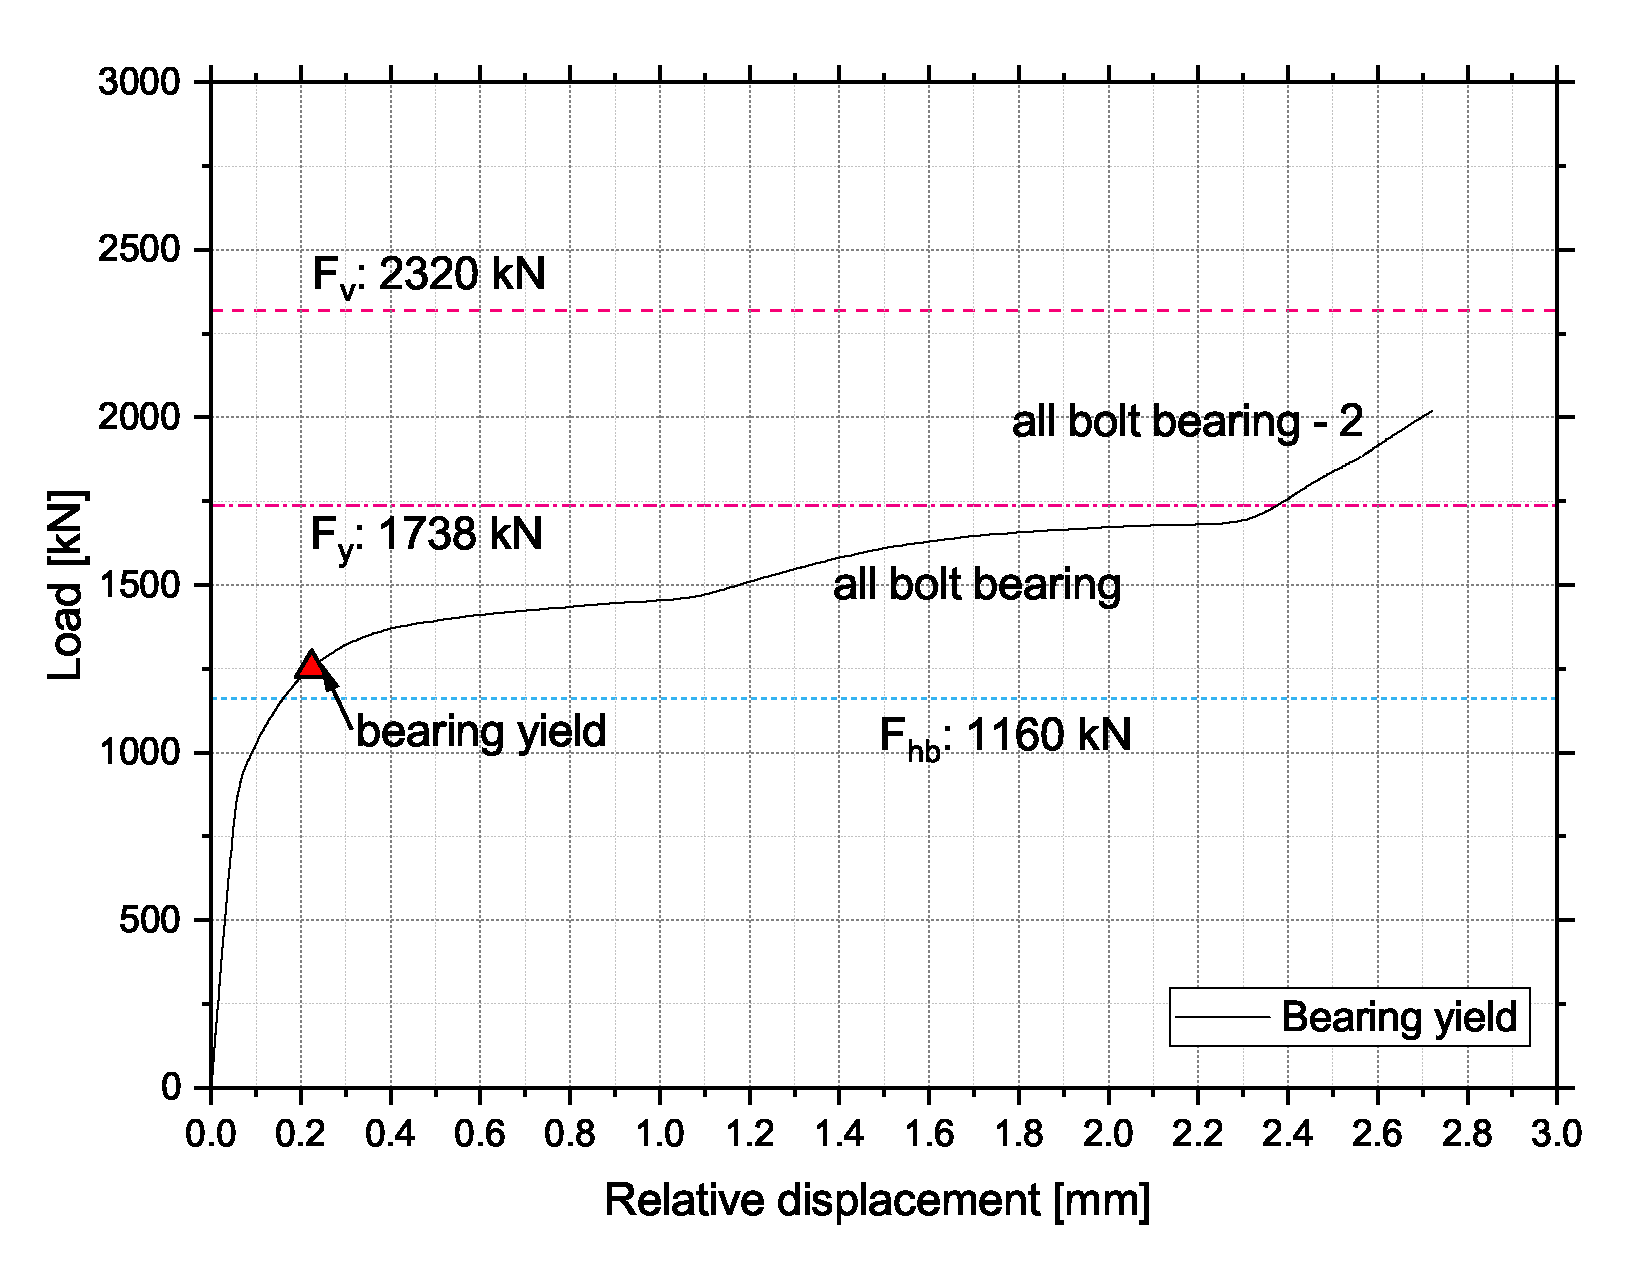
\includegraphics[width=0.7\textwidth]{imgs/ch7/b4s40t30.eps}
    \caption{The relationship between load and relative displacement for bearing yield first case.}
    \label{fig-beafst}
\end{figure}

Fig. \ref{fig-beafstcp} shows the Mises stress counter of the joint for bolts (thickness center of main plate, Maximum = 900 Mpa, when load = 1251 kN), Fig. \ref{fig-beafstcp-2} shows the Mises stress counter of the joint for the main plate (faying surface of the main plate, Maximum stress = 235 Mpa, when load = 1251 kN), From the figure, it can be found that when the load is equal to 1251 kN, the whole cross-section within the bearing contact range of the main plate has yielded, and it can be assumed that the joint has yielded under pressure, and at this time, the joint is in the limit state of yielding under pressure, and with reference to Fig. \ref{fig-beafst}, it can be found that the curve is experiencing a nonlinear change at this time, and it is about to enter into the stage of plastic ductility.

Fig. \ref{fig-beafstcp} shows the Mises stress counter of the joint for the plate (thickness center of main plate, Maximum stress = 900 Mpa, when load = 1251 kN). Against Fig. \ref{fig-beafst}, it can be seen from this figure that it is not the yielding of the shear plane of the bolt that causes the curve to go into a nonlinear behavior, so this state can be ruled out.

\begin{figure}[htbp]
    \centering
    \begin{minipage}[t]{0.8\textwidth}
    \includegraphics[width=\linewidth]{imgs/ch7/beafst-count-p.png}
    \caption{Mises stress counter of the joint for bolts (thickness center of main plate, Maximum stress = 235 Mpa, when load = 1251 kN)}
    \label{fig-beafstcp}
    \end{minipage}
    \begin{minipage}[t]{0.8\textwidth}
    \includegraphics[width=\linewidth]{imgs/ch7/beafst-scout-mp.png}
    \caption{Mises stress counter of the joint for the main plate (faying surface of the main plate, Maximum stress = 235 Mpa, when load = 1251 kN)}
    \label{fig-beafstcp-2}
    \end{minipage}
    \begin{minipage}[t]{0.8\textwidth}
    \includegraphics[width=\linewidth]{imgs/ch7/beafst-count-b.png}
    \caption{Mises stress counter of the joint for the plate (thickness center of main plate, Maximum stress = 900 Mpa, when load = 1251 kN)}
    \label{fig-beafstcb}
    \end{minipage}
    \label{fig-beafstc}
\end{figure}



\subsubsection{Reduction factor}

Fig. \ref{fig-beafstls} shows the Decline ratio of bolt preload when load is equal to the 1251 kN (bearing yield first case). From the figure, it can be seen that when it is judged as bearing yielding, since the nonlinear behavior of the joint arises around the bolt holes of the main plate, there is not much effect on the shaft of the bolt, and the bolt shaft as a whole is still in the linear elasticity stage, so the preload of the bolt does not change significantly as in the case of shear yielding case. Although the preload still drops to about 0.9, this value is very small for the whole, so it is considered here that the correction factor for the slip strength regarding the preload can be disregarded for the bearing resistance yield case.

\begin{figure}[htbp]
    \centering
    \includegraphics[width=0.7\textwidth]{imgs/ch7/b4t30w27-ls.eps}
    \caption{Decline ratio of bolt preload when load is equal to the 1251 kN (bearing yield first case)}
    \label{fig-beafstls}
\end{figure}


\subsubsection{Summary}

For the bearing yield limit state, since the occurrence of nonlinear behavior depends around the main plate fastener holes, the fasteners used for bearing connections are also not subjected to excessive shear resulting in a loss of preload, however, like the shear yield mode, the friction located in the if the front end is configured with a fastener used for a bearing type of connection, which produces a moment due to shear, will cause the main plate to deform and will still result in a friction force Therefore, it is not recommended to take into account the friction of bolt (b1) at the front end for such cases. The reduction factor due to the uneven distribution of loads in the bearing connection is still applicable to bearing resistance, therefore it is still recommended to multiply this reduction factor $\beta_{ls}$ when calculating the bearing yield resistance $F_{hv}$.

For SLS:
if bearing type connection is arranged at the front end of the joint :

\begin{equation}
\begin{aligned}
    F_{hb} &= (n-1) F_s + \beta_{ls} n_b F_{by1}\\
           &= (n-1) F_s + 0.9 n_b F_{by1}
\end{aligned}
\end{equation}

if not :

\begin{equation}
\begin{aligned}
    F_{hb} &= n F_s + \beta_{ls} n_b F_{by1}\\
           &= n F_s + 0.9 n_b F_{by1}
\end{aligned}
\end{equation}

For ULS, see other specifications such as Eurocode 3:

\begin{equation}
    F_v = n k_m \alpha_b d t f_{u}
\end{equation}


\subsection{Net cross-section yield}

For the net interfacial yield strength of the main slab, the method of calculation has not changed from the recommendations given in the various codes and is calculated according to the following equation.

\begin{equation}
    F_y = (w-d_0) t f_y
\end{equation}


\section{Summary}

For hybrid joints with friction and bearing connections, the service limit states can be categorized as: a.Shear yield limit state for the fastener shaft, b. Bearing yield limit state for main plate, c. Net cross-section yield limit state as shown in Fig. \ref{fig-schehysls}.

\begin{figure}[htbp]
    \centering
    \includegraphics{imgs/ch7/sche-hy-sls.pdf}
    \caption{Schematic of the yield mode on the serviceability limit state}
    \label{fig-schehysls}
\end{figure}

Table\ref{tab-sumeq} summarizes the calculate equation for the hybrid joint on the serviceabilit limit state.

Hybrid joints mainly take into account the loss of preload due to shearing of the fasteners and the loss of friction of the fasteners located at the ends, in addition to the proposed discount factor due to the uneven distribution of loads in the bearing connection.

\begin{table}[htbp]
\centering
\caption{Calculate equation for hybrid joint on the SLS} \label{tab-sumeq}
\begin{tabular}{@{}lcc@{}}
\toprule
\multicolumn{3}{c}{Serviceability limit state}                                                  \\ \midrule
\multicolumn{1}{c}{} & \begin{tabular}[c]{@{}c@{}}If b1 arranged \\ fastener for bearing\end{tabular} & \begin{tabular}[c]{@{}c@{}}If \\ not\end{tabular} \\ \cmidrule(l){2-3} 
\begin{tabular}[c]{@{}l@{}}Shear yield resistance\\ for fastener shaft $F_{hv}$\end{tabular} &$(n_f+ \alpha_v(n_b-1)) F_s + \beta_{ls} n_b F_{vy1}$ & $(n_f+ \alpha_v n_b) F_s + \beta_{ls} n_b F_{vy1}$ \\
\begin{tabular}[c]{@{}l@{}}Bearing yield resistance\\ for main plate $F_{hb}$ \end{tabular}   & $(n-1) F_s + \beta_{ls} n_b F_{by1}$ & $ n F_s + \beta_{ls} n_b F_{by1}$ \\
\begin{tabular}[c]{@{}l@{}}Net cross-section yield\\ resistance $F_y$\end{tabular}   & \multicolumn{2}{c}{$ (w-d_0) t f_y$} \\ \bottomrule
\end{tabular}
\end{table}

Where, $\alpha_v$ is Correction factor for loss of preload due to shear failure, $\beta_{ls}$ is the correction factor for load sharing. $n$ is the number of the fastener, $n_f$ is the number of the fastener for friction type connections, $n_b$ is the number of the fastener for bearing type connections, $F_{by1}= dtf_y$, $F_{vy1} = A_s f_{yb}/\sqrt{3}$.

In addition, the reduction factor due to the conversion of static friction to kinetic friction should also be considered. However, the loading rate required for the conversion of static friction to kinetic friction varies according to the joint processing conditions, so in order to simplify the calculations, the friction coefficient can be considered as a factor of slip instead of slip coefficient for calculating the slip strength, and this topic will be discussed in the future to calculate the reliability of the calculation based on the coefficient of friction.

For the limit states, it is considered sufficient to follow the existing methods of strength calculation and classification. The only difference is that since all fasteners do not enter the bearing connection at the same time, fasteners that enter the bearing connection at the beginning may fail prematurely due to early entry into the bearing state, and therefore the strength of the limit states of the hybrid connection may be considered to require a reduction factor.